
\section{Imaginou? Agora só vem}

Uma vez ouvi a seguinte frase dita por Gustavo Caetano\footnote{CEO da SambaTech} que nunca mais saiu de minha mente:
\begin{quote}
    \textbf{SE} você me traz um problema \\
    \textbf{MAS} não me traz a solução \\
    \textbf{ENTÃO} você faz parte do problema
\end{quote}

Depois de refletir por muito tempo, entendi que nem sempre sabemos a solução de todos os problemas assim quando nos deparamos com eles e que todos os problemas devem ser reportados imediatamente para mitigar quaisquer efeitos colaterais. Por isso, tomei a liberdade de adaptar essa frase para algo um pouco mais tangível:
\begin{quote}
    \textbf{SE} você me traz um problema \\
    \textbf{ENTÃO} vamos discutir uma solução \\
    \textbf{POIS} juntos trabalhamos melhor
\end{quote}

Baseado nessa frase, gostaria de apresentar uma metodologia ágil que estou desenvolvendo para reconstrução de processos maduros a qual batizei de \textbf{AIOROS}\footnote{Cavaleiro de Ouro de Sagitário que morre para salvar a Princesa Athena}. Por mais caricata ou incomum que pareça, esta metodologia foi baseada na série japonesa de mangá chamada \textbf{Os Cavaleiros do Zodíaco} veiculada no Brasil por volta dos anos 90 mas que se encaixa muito bem como analogia na reconstrução de sistemas legados.

Apesar de possuir diversas sagas, é a primeira que nos interessa por fazer uma analogia quase perfeita para com o contexto que precisamos, onde os cavaleiros de bronze precisam salvar a princesa ferida, correndo contra o tempo onde precisam passar pelas 12 casas do zodíaco enfrentando seus guardiões.

\begin{figure}[H]
    \centering
    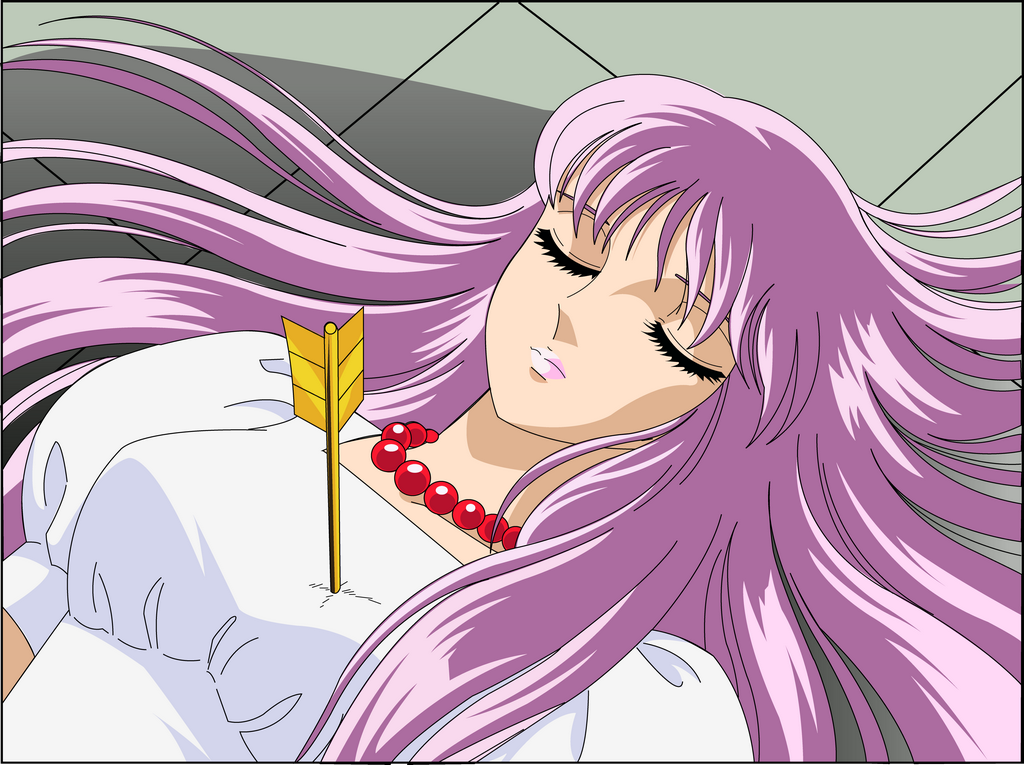
\includegraphics[scale=0.33,keepaspectratio=true]{images/08.png}
    \caption{Saori ferida, reencarnação de Athena}
    \label{pic_08}
\end{figure}

Adaptando essa estória para nossa realidade, imagine que a princesa Saori seja a empresa ou o processo que está em execução de forma legada, ou seja, apenas desempenhando sia função básica não sendo capaz de entregar nada além disso. Ver Figura \ref{pic_08}.

\begin{figure}[H]
    \centering
    
\includegraphics[scale=0.33,keepaspectratio=true]{images/09.jpg}
    \caption{Os Cavaleiros de Bronze}
    \label{pic_09}
\end{figure}

Já os cavaleiros de bronze (Figura \ref{pic_09}) representam os funcionários treinados e prontos para colocar as mãos na na massa e reconstruir todo aquele software ou processo legado que não os deixavam evoluir ou gerava muito retrabalho como tickets ou pequenos incrementos ou correções.

\begin{figure}[H]
    \centering
    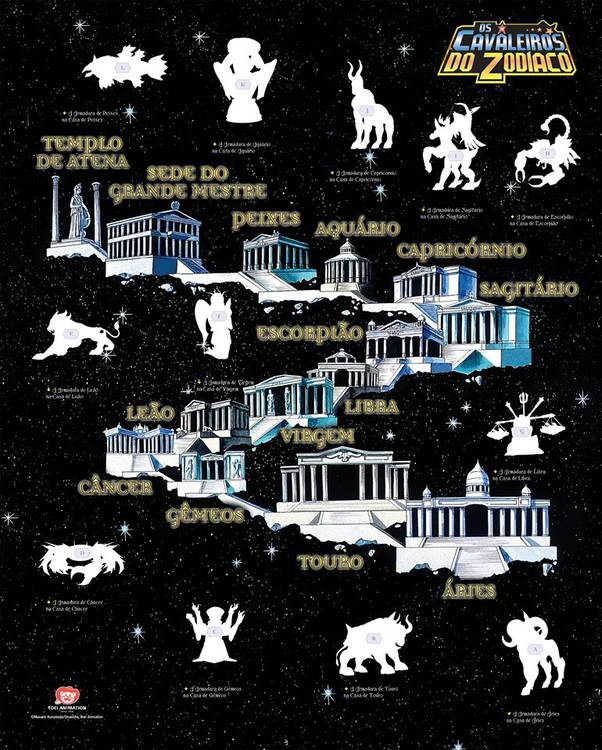
\includegraphics[scale=0.55,keepaspectratio=true]{images/10.jpg}
    \caption{As 12 casas do Zodíaco}
    \label{pic_10}
\end{figure}

As 12 Casas do Zodíaco (Figura \ref{pic_10}) representam em quantas partes o processo como um todo deverá ser quebrado. A quantidade de casas depende muito do sistema que esteja sendo reconstruído: 
\begin{itemize}
    \item Poucas casas deixam o sistema muito coeso, de difícil manutenção e com Cavaleiros de mais para combater
    \item Muitas casas deixam o sistema muito esparso, de difícil manutenção e com Cavaleiros de menos para combater
\end{itemize}
O segredo é ter uma equipe experiente para se definir qual é o número ideal de casas.

Aqui observamos um fenômeno curioso: mem todos cavaleiros precisam lutar em todas as casas ao mesmo tempo. Geralmente fica um pequeno time atuando em uma casa e os demais times se espalham em outras casas que fazem mais sentido a eles. Ou seja,  este processo pode ser altamente paralelizável desde que haja uma floresta de dependência árvores distintas para que se haja a maior quantidade de podas possível. 

\begin{figure}[H]
    \centering
    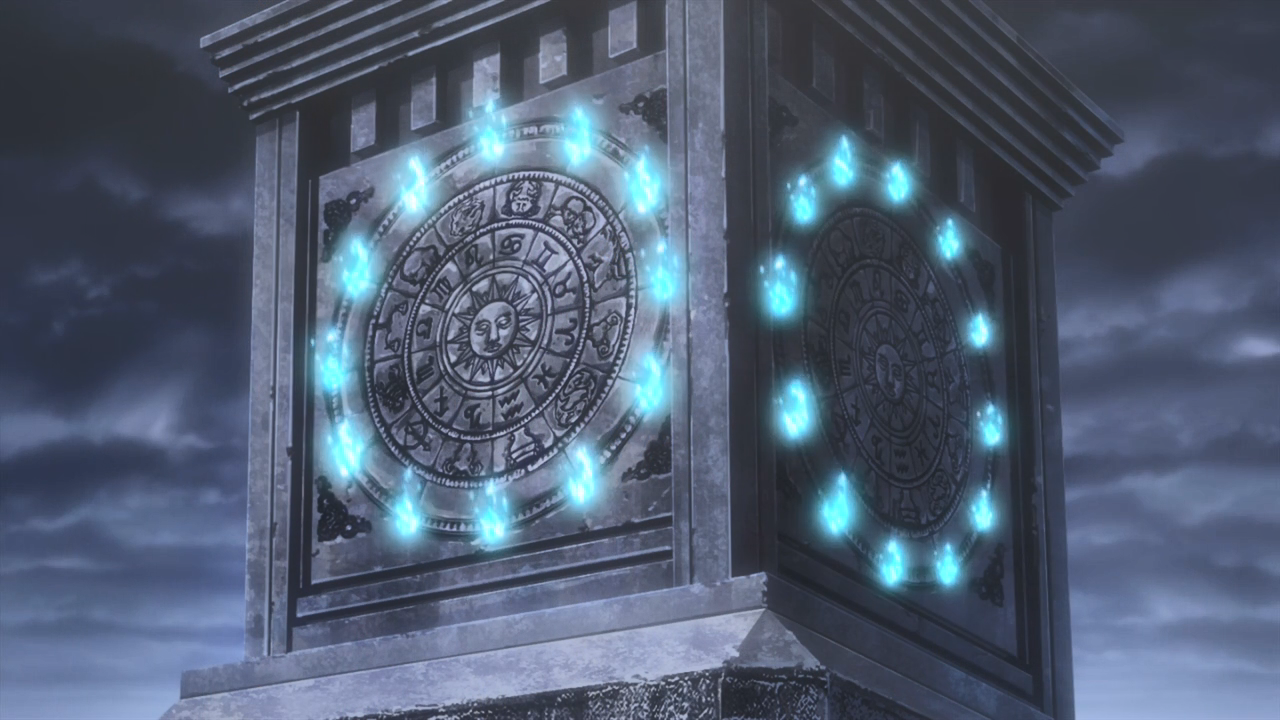
\includegraphics[scale=0.35,keepaspectratio=true]{images/11.png}
    \caption{Relógio das 12 casas do Zodíaco}
    \label{pic_11}
\end{figure}

O Relógio do Zodíaco, Figura \ref{pic_11}, representa a agilidade, ou seja, o time não tem muito tempo a perder pois processos, funcionários e clientes como um geral aguardam  por melhorias e o time deve trabalhar de forma integrada, coesa, a fim de garantir essa entrega no prazo.

Um pequeno resumo de como o Pilar do Conhecimento poderia trabalhar para entregar valor:
\begin{enumerate}
    \item Reunião inicial a fim de explicar a todos o que será feito daqui pra frente;
    \item Segunda reunião com os membros mais experientes para se definir quais serão as casas a serem e seus guardiões (deve-se haver pelo menos 2 guardiões para que haja uma cooperação mútua)\footnote{um guardião pode defender mais de uma casa};
    \item Os guardiões devem definir as regras de negócio e os critérios de aceite das suas casas.
    \item Agora é a vez dos cavaleiros utilizarem do que há de melhor, elevando seus cosmos ao sétimo sentido, propondo soluções engenhosas capazes de cobrir tudo que foi proposto pelos guardiões daquela casa. 
    \item Neste momento, Product Managers, Designers e Writers atuam ativamente na composição da solução do produto.
    \item Estes passos devem ser repetidos até que todo o projeto tenha finalizado. 
    \item Agora, Product Managers, Designers e Writers devem dar um formato ao projeto, adicionando Epic, História e Tarefa para que os times executantes possam indicar o esforço para cada tarefa descrita. 
    \item Writers, não devem se esquecer de que faz parte da entrega todas as chaves estarem traduzidas quando o projeto estiver fechado, ou seja, o time de desenvolvimento não poderá iniciar qualquer tarefa desde que essa condição não seja satisfeita. Essa entrega pode ser feita via arquivo de texto anexado no card do jira, por exemplo.
    \item Voltando a falar sobre mensurar, como já teremos nosso livro de playbook, teremos uma grande noção do quanto dura cada atividade, pelo menos uma boa aproximação. Dessa forma, fica bem mais simples e preciso saber quando uma tarefa deverá ser finalizada.
\end{enumerate}
